%-----------------------------------------------------------------------------%
% Format and styling in this file originally created by 
% Carl E. Svensson 2010, updated by Adam J. Carmichael 2011
%-----------------------------------------------------------------------------%
%
%- Document Makeup -----------------------------------------------------------%
%- (01) Notes from template author
%- (02) Document Class and Options
%- (03) Standard package includes and options
%- (04) Custom Definitions and Alterations
%- (05) Custom Commands
%- (06) Document title and other metadata
%- (07) Start Document Content
%- (07a) Misc Config
%
%
%- (01) Notes from carneeki@ -------------------------------------------------%
% NEATNESS:
%  Please keep the TeX neat. Best ways to do this:
%  (01) Don't indent
%  (02) Keep inside of 80 characters (it makes for nicer editing on small
%       laptops).
%  (03) Avoid whitespace between \section{} and other document elements. We
%       have %%%% comments for a reason!
%  (04) Use 2 (that's TWO) space characters to indent. NEVER use tab unless
%       your editor converts to to space chars.
%  (05) Maintain customisations in their respective sections.
%  (06) Comment everything. Bandwidth and diskspace are cheap these days, and
%       TeX compresses pretty nice. Anything else is the BAD kind of laziness
%       on your part.
%
% MULTILINE EQUATIONS:
%  Use \begin{align} instead of \begin{eqnarray}...
%  Details as to why are found at (tl;dr : it's just better...):
%  http://texblog.net/latex-archive/maths/eqnarray-align-environment/
% 
% BIBLIOGRAPHY: 
%  -> URLS: to generate the GUID for a reference that is for a URL, paste
%     the URL into goo.gl and then take only the suffix portion.
%
%  -> Wikipedia citations, simply copy + paste the citation from the
%     menu on the LHS.
%
%
%- (02) Document Class and Options -------------------------------------------%
\documentclass[
%  pagesize,
  a4paper,
  pdftex,
%  fontsize=11pt,
  draft=false,
  twoside,
]{book}
%
%
%- (03) Standard package includes and options --------------------------------%
%\usepackage{draftwatermark} % draft watermark. Comment these 2 lines in final
%\SetWatermarkLightness{0.9} %
\usepackage{amsmath}       % amsmath & amssymb are almost ALWAYS required.
\usepackage{amssymb}       %
%
%\usepackage{verbatim}     % multiline commenting ( c++ equiv /* ... */ )
%
\usepackage{xcolor}         % pdflatex
\definecolor{neekiRed}{RGB}{172,40,41}
\definecolor{neekiBlue}{RGB}{62,70,157}
%
\usepackage{geometry}      % option for altering page dimensions if needed
\usepackage[pdftex]{graphicx} % including image files for figures (ie
                              % non-[E]PS)
%                          % valid types: jpeg, png, pdf
\usepackage{wrapfig}       % the figures themselves
\usepackage[numbers,
square,
longnamesfirst
]{natbib}                  % prettybib
\usepackage[pdftex]{hyperref} % clickable TOC and refs
\usepackage[all]{xy}      % category theory helpers
\xyoption{all}            % category theory helpers
\input xy                 % category theory helpers
\usepackage{tikz}        % easy graphic thing
\usetikzlibrary{arrows,shapes,positioning}
\usepackage{tabularx}    % easy tables
\usepackage{url}         % easy urls
\usepackage{multirow}    % 
\usepackage{lipsum}      % autogen placeholder text
%
%- (04) Custom Definitions and Alterations -----------------------------------%
\usepackage[T1]{fontenc} % font-doohickey
%\usepackage{tgadventor}  % font
%\usepackage[math]{iwona} % font
\usepackage[light,math]{kurier} % font
%
\linespread{1.5} % carneeki@ use approx 150% line spacing just like MaxDesign.
\hypersetup{
  % DO NOT CHANGE THESE
%   pdftitle={\metaTitle},
%   pdfauthor={\metaAuthorShort},
%   pdfsubject={\metaSubject},
%   pdfkeywords={\metaKeywords},
  pdfcreator={LaTeX},
  pdfproducer={LaTeX},
  pdftoolbar=false,
  % But change these to taste:
  pdffitwindow=false,   % window fit to page when opened
  pdfstartview={Fit},   % fits the width of the page to the window
                        % all (useful) opts: Fit, FitH, FitV,
  pdfnewwindow=true,    % open links in new window
  colorlinks=true,      % false = boxed links; true = colored links
  linkcolor=neekiRed, % color of internal links
  citecolor=neekiBlue, % color of links to bibliography
  filecolor=red, % color of file links
  urlcolor=red  % color of external links
}
%
%- (05) Custom Commands ------------------------------------------------------%
\newcommand{\derivative}[1][x]{\frac{\mathrm{d}}{\mathrm{d}#1}}
\newcommand{\lxor}{\oplus}
\newcommand{\lxnor}{\lnot\lxor}
\newcommand{\neqref}[1]{\text{(#1)}}
\newcommand{\true}{(\mathbb{T})}
\newcommand{\false}{(\mathbb{F})}
%
%- (06) Document Title and other metadata ------------------------------------%
%
\title{
  Grokking DMTH137
}
%
\author{
  Adam J. Carmichael \\
  Undergraduate Student \\
  Department of Electronic   Engineering\\
  Macquarie University\\
  Sydney, Australia 2109\\
  Email: \url(adam.carmichael@ieee.org) \\
} % author END Brace
%
%- (07) Start Document Content -----------------------------------------------%
\begin{document}
%- (07a) Misc Config ---------------------------------------------------------%
%-----------------------------------------------------------------------------%
%\cfoot{\thepage\ of \pageref{LastPage}} % page n of m
%
\maketitle
%
%\begin{abstract}
% This document forms the notes for DMTH137 by the author. DMTH137 changed from
% programming in C++ to programming in Java however the essence of DMTH137
% syllabus the same. It is about linked data structures. 
%\end{abstract}
%
\section{Introduction}
\label{sec:Introduction}
DMTH137 is about data structures and algorithms.
%-----------------------------------------------------------------------------%
%- Table of Contents ---------------------------------------------------------%
%-----------------------------------------------------------------------------%
\tableofcontents
%
\newpage

%-----------------------------------------------------------------------------%
%- Networks ------------------------------------------------------------------%
%-----------------------------------------------------------------------------%
\chapter{Networks}
\label{chap:Networks}
%-----------------------------------------------------------------------------%
%- Networks :: Undirected and Directed Graphs --------------------------------%
%-----------------------------------------------------------------------------%
\section{Undirected and Directed Graphs}
\label{sec:UndirectedAndDirectedGraphs}

We are used to graphs are often used to describe functions such as $y = f(x)$.
We will not be using them in DMTH137.

It is important to note that a graph is a collection of points
called ``\emph{vertices}'' and lines or connections which join them called
``\emph{edges}''.

A vertex can represent a piece of information and the edge represents how they
are connected.

Example: A vertex represents people and the edges represent the degrees of
separation to which they know eachother.

Example: Each vertex represents a town and the edge represents the distance
between each town.

\emph{Edges must join two distinct vertices}. A graph with loops allows an edge
to join a vertex to itself. (If you have had Cisco switching experience: compare to the
packet storm created in a switched network without spanning tree protocol
implemented).

There are two types of graphs we look at in DMTH137:
\begin{enumerate}
  \item Directed graphs
  \item Undirected graphs
\end{enumerate}

A directed graph has arrows along the edges to indicate the flow of the
direction. Undirected graphs have no arrows. An arrow may point one way, the
opposite way, or double arrows to indicate bidirectionality.

% TODO: include example of directed graph ( ->, <-, <-> )

% TODO: include example of undirected graph 

Sometimes a graph (be it directed or undirected) will have a number or
\emph{weight} with an edge, and is written next to the edge itself.

% TODO: include example of weighted graph.

In terms of language, we say ``Vertex A is adjacent to Vertex B if there is an
edge from A to B''.

\subsection{Equivalence in Graphs}
How do we know when two graphs are the same graph?

When the vertices in one graph, GraphA are able to be translated to a second
graph, GraphB such that both sets of vertices are joined in the same way.

$ A-> (B,C,D) $ % TODO: let this be a messy graph of spaghetti.
$ 1-> (2,3,4) $ % TODO: let this one look like Bruce Schneir's alphabet soup
(through his eyes)

There is only one graph with a single vertex:
% TODO: draw a single vertex
\begin{tikzpicture}
\end{tikzpicture}


2 Vertices:
% TODO: draw 2 points
% TODO: draw 2 points connected

3 vertices:
% TODO: draw 3 points
% TODO: draw 3 points with 2 points connected
% TODO: draw 3 points with 3 points connected

4 vertices:
% TODO: draw 4 points
% TODO: draw 4 points with 2 points connected
% TODO: draw 4 points with 3 points connected 
  % TODO: draw 4 points with 3/4 box
  % TODO: draw 
% TODO: draw 4 points with 4 points connected
  % TODO: draw 4 points as box
  % TODO: draw 4 points with 3/4 box and 1 diagonal

% TODO: just refer to the photos...

Complete graph:

$K_n$ - the complete graph of n vertices is the graph of n vertices
where every pair of vertices is adjacent

$K_3$ (3 points; draw a triangle); 3 edges
$K_4$ (4 points; draw a square and a bend); 5 edges
$K_5$ (5 points; draw a pentagram in a pentagon); 10 edges

Bipartite graph
% TODO: refer to photos
$K_(n,m)$

$K_(3,4)$ (a graph in 2 parts) % bipartite

$K_(3,2)$



%-----------------------------------------------------------------------------%
%- Networks :: Spanning Trees and Traversal Strategies -----------------------%
%-----------------------------------------------------------------------------%
\section{Spanning Trees and Traversal Strategies}
\label{chap:SpanningTreesAndTraversalStrategies}
%-----------------------------------------------------------------------------%
%- Networks :: Walks, Paths and Cycles ---------------------------------------%
%-----------------------------------------------------------------------------%
\section{Walks, Paths and Cycles}
\label{sec:WalksPathsCycles}

An \emph{Eulerian path} is a path in a graph which includes every edge.
An \emph{Eulerian circuit} is an Eulerian path which begins and ends at the same
vertex.

Can an Eulerian path be found on the diagram of ``The 7 Bridges of Konigsber''?

% following diagram courtesy of:
% http://www.texample.net/tikz/examples/bridges-of-konigsberg/
\begin{center}
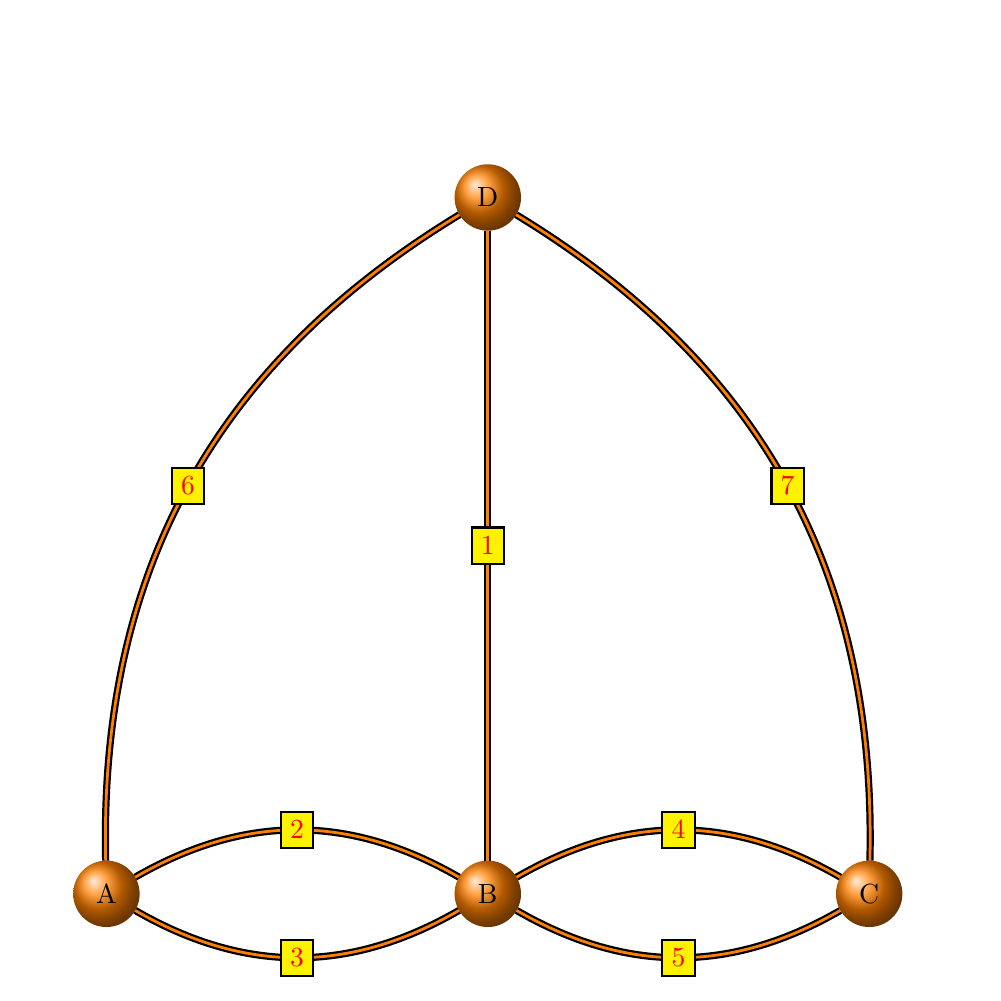
\begin{tikzpicture}[node distance   = 4 cm]
  \useasboundingbox (-1,-1) rectangle (11,11); 
  \tikzset{VertexStyle/.style = {shape          = circle,
                                 ball color     = orange,
                                 text           = black,
                                 inner sep      = 2pt,
                                 outer sep      = 0pt,
                                 minimum size   = 24 pt}}
  \tikzset{EdgeStyle/.style   = {thick,
                                 double          = orange,
                                 double distance = 1pt}}
  \tikzset{LabelStyle/.style =   {draw,
                                  fill           = yellow,
                                  text           = red}}
     \node[VertexStyle](A){A};
     \node[VertexStyle,right=of A](B){B};
     \node[VertexStyle,right=of B](C){C};
     \node[VertexStyle,above= 8 cm of B](D){D};     
     \draw[EdgeStyle](B) to node[LabelStyle]{1} (D) ;
     \tikzset{EdgeStyle/.append style = {bend left}}
     \draw[EdgeStyle](A) to node[LabelStyle]{2} (B);
     \draw[EdgeStyle](B) to node[LabelStyle]{3} (A);
     \draw[EdgeStyle](B) to node[LabelStyle]{4} (C);
     \draw[EdgeStyle](C) to node[LabelStyle]{5} (B);
     \draw[EdgeStyle](A) to node[LabelStyle]{6} (D);
     \draw[EdgeStyle](D) to node[LabelStyle]{7} (C);

  \end{tikzpicture}
\end{center}

\emph{No}. The number of times you enter a circuit equals the number of times
you leave. Each time you enter, you use a different edge. If you enter a vertex
twice, you would have to have used that same entrance twice. Every time you
leave, it is via a different and unused edge.



%-----------------------------------------------------------------------------%
%- Networks :: Direct Proofs and Proofs By Contradictions --------------------%
%-----------------------------------------------------------------------------%
\section{Object Oriented Design and Development}
\label{chap:ObjectOrientedDesignandDevelopment}
\lipsum[1]

%-----------------------------------------------------------------------------%
%- Networks :: Modular Arithmetic --------------------------------------------%
%-----------------------------------------------------------------------------%
\section{Modular Arithmetic}
\label{chap:ModularArithmetic}

%-----------------------------------------------------------------------------%
%- The Natural Numbers and Mathematical Induction ----------------------------%
%-----------------------------------------------------------------------------%
\section{The Natural Numbers and Mathematical Induction}
\label{chap:NaturalNumbersAndMathematicalInduction}

%-----------------------------------------------------------------------------%
%- Prime Numbers and Factorisation -------------------------------------------%
%-----------------------------------------------------------------------------%
\section{Prime Numbers and Factorisation}
\label{sec:PrimeNumbersAndFactorisation}

%-----------------------------------------------------------------------------%
%- Greatest Common Divisors and Least Common Multiples -----------------------%
%-----------------------------------------------------------------------------%
\section{Greatest Common Divisors and Least Common Multiples}
\label{sec:GCDandLCM}

%-----------------------------------------------------------------------------%
%- Euclid's Algorithm
%-----------------------------------------------------------------------------%
\section{Euclid's Algorithm}
\label{sec:EuclidsAlgorithm}

%-----------------------------------------------------------------------------%
%- Chinese Remainder Theorem
%-----------------------------------------------------------------------------%

%-----------------------------------------------------------------------------%
%- Logic
%-----------------------------------------------------------------------------%
\chapter{Logic}
\label{chap:Review}

%-----------------------------------------------------------------------------%
%- Logic :: Propositional Logic and Truth Tables
%-----------------------------------------------------------------------------%
\section{Propositional Logic and Truth Tables}
\label{sec:PropositionalLogicAndTruthTables}

A proposition is a statement that is either true or false.

``It is Thursday'' is a statement, which may be true or false depending on the
day.
``Pigs can fly'' is a statement, which is most likely false unless something odd
is done to the pig.
$2 + 3 = 5$ is a statement which turns out to be true (T).
$2 + 3 = 7$ is a statement which turns out to be false (F).
$ -3 < 7  $ (T)
$\frac{5}{4} > \frac{6}{5}$ (T)

Some things which are not propositions:
\begin{itemize}
  \item ``Go away.'' is a statement, but cannot be resolved to a true or false
  value. ``Because it's Monday''. This is only a sentence fragment 
  \item $ x + y $
  \item ``I am lying.'' is a paradox. If you actually are lying, then the
  statement is true and thus no longer a lie (and hence the truth). Paradoxes come about due to
the notion of ``self-reference''.
  \item ``This sentence is false'' is another example. Interestingly though,
  ``This sentence is true'' is not a paradox.
  \item ``Nothing is true'' is another paradox \footnote{and is an oft used
  topic in post-modernism, but that's arts topic and best left to people who
  belong in Y3A}.
  \item Russell's Paradox
\end{itemize}

Most things that we want to say contain more than a single idea so we must
combine, so we must combine propositions in some way.

Propositions are often represented by the letters p and q. They can be combined
using things called ``connectives'' like:
\begin{itemize}
  \item and
  \item or
  \item not
  \item xor
  \item xnor
  \item implies
  \item iff (if and only if)
  \item equivalent
\end{itemize}

Let ``p'' be the statement ``I like tea'' and ``q'' be the statement ``I like
coffee''.

If I wanted to say: ``I like tea and coffee'': $p \land q$
If I wanted to say: ``I like tea or coffee'': $p \lor q$
If I wanted to say: ``I like tea but not coffee'': $p \land \lnot q$
``I don't like tea or coffee'' can be written two ways: $ -(p \lor q)$ or $\lnot p
\land \lnot q $

Let ``p'' be the statement ``It is raining.''
Let ``q'' be the statement ``I need an umbrella.''

If it is raining, then I need an umbrella:

$ p \to q $

ie, the fact that it is raining implies that I need an umbrella.

If it is not raining, so I don't need an umbrella.

$ \lnot p \to \lnot q $

What about $q \to p$?
This says: ``If I need an umbrella, then it is raining.'' This is not
necessarily true as there may be many uses for an umbrella besides keeping rain
off\footnote{eg an umbrella salesman or as a parachute}.

Let ``p'' be the statement ``he is vegetarian''
Let ``q'' be the statement ``he eats no meat''

He is vegetarian if and only if he eats no meat.

$ p \iff q \equiv (p -> q) \land (q -> p)$
This establishes equivalence between proposition p and q.


Conjunction $p \land q$ is true only when both p,q are true.
\begin{table}[!htb]
\label{tab:TruthTableAND}
\begin{tabularx}{\linewidth}{| c | c | X |} \hline
  p & q & $(p \land q)$ \\ \hline \hline
  F & F & F \\ \hline
  F & T & F \\ \hline
  T & F & F \\ \hline
  T & T & T \\ \hline
\end{tabularx}
\caption{Truth Table: logical AND}
\end{table}

Disjunction $p \lor q$ is true when at least one of p,q are true:
\begin{table}[!htb]
\label{tab:TruthTableOR}
\begin{tabularx}{\linewidth}{| c | c | X |} \hline
  p & q & $(p \lor q)$ \\ \hline \hline
  F & F & F \\ \hline
  F & T & T \\ \hline
  T & F & T \\ \hline
  T & T & T \\ \hline
\end{tabularx}
\caption{Truth Table: logical OR}
\end{table}

Negation $\lnot p$ is true when $p$ is false
\begin{table}[!htb]
\label{tab:TruthTableNOT}
\begin{tabularx}{\linewidth}{| c | X |} \hline
  p & $(\lnot p)$ \\ \hline \hline
  F & T \\ \hline
  T & F\\ \hline
\end{tabularx}
\caption{Truth Table: logical NOT}
\end{table}

Conditional $p \to q$ if p then q, or ``p implies q''. This is false when
$p$ is true and $q$ is false with a default condition of true.

\begin{table}[!htb]
\label{tab:TruthTableIMPLIES}
\begin{tabularx}{\linewidth}{| c | c | X |} \hline
  p & q & $(p \to q)$ \\ \hline \hline
  F & F & T \\ \hline
  F & T & T \\ \hline
  T & F & F \\ \hline
  T & T & T \\ \hline
\end{tabularx}
\caption{Truth Table: logical IMPLIES}
\end{table}

A plain English example: It can't rain when there are no clouds, so ``if it is
raining then it is not cloudy'' is false.

Suppose it isn't raining, it could still be cloudy. This remains true.

Converse $q \to p$
\begin{table}[!htb]
\label{tab:TruthTableCONVERSE}
\begin{tabularx}{\linewidth}{| c | c | X |} \hline
  p & q & $(q \to p)$ \\ \hline \hline
  F & F & - \\ \hline
  F & T & - \\ \hline
  T & F & - \\ \hline
  T & T & - \\ \hline
\end{tabularx}
\caption{Truth Table: logical CONVERSE}
\end{table}

If it is cloudy then it is raining (not always true).
q->p is NOT the same as $p -> q$

Contrapositive $\lnot p -> \lnot q$
Use to establish the notion of ``proof by contradiction''.

Double conditional $ p \equiv q $
p if and only if q: p iff q
$p \to q$ and $q \to p$ must both be true
That is $(p \equiv q) \equiv (( p \to q) \land (q \to p))$

\begin{table}[!htb]
\label{tab:TruthTableEQUIVALENCE}
\begin{tabularx}{\linewidth}{| c | c | X |} \hline
  p & q & $( p \equiv q ) \equiv (( p \to q) \land (q \to p))$
                                                    \\ \hline \hline
  F & F & F \\ \hline
  F & T & F \\ \hline
  T & F & F \\ \hline
  T & T & T \\ \hline
\end{tabularx}
\caption{Truth Table: logical DOUBLE CONDITIONAL}
\end{table}

eg let p: 4 is an even number
       q: 4 is divisible by 2
       p and q clearly mean the same thing.
       
Exclusive or (xor) $p \lxor q$
This is true when either p,q is true, but not both.

\begin{table}[!htb]
\label{tab:TruthTableXOR}
\begin{tabularx}{\linewidth}{| c | c | X |} \hline
  p & q & $( p \lxor q )$ \\ \hline \hline
  F & F & F \\ \hline
  F & T & T \\ \hline
  T & F & T \\ \hline
  T & T & F \\ \hline
\end{tabularx}
\caption{Truth Table: logical XOR}
\end{table}

How large should you make your truth table?
\begin{enumerate}
  \item For every variable we have 2 possible values: True and False.
  \item If we have n propositions we need ${2}^{n}$ rows in the truth table.
\end{enumerate}
For example, if we have the variables $p,q,r$ then we need ${2}^{3} = 8$ rows.

% TODO: fix order of operations

Order of operations:

\begin{enumerate}
  \item Do OR connectives
  \item Do AND connectives
\end{enumerate}


Two expressions are logically equivalent if their truth values match for every
combination of the truth values of their atomic propositions\footnote{an atomic
proposition is a proposition cannot be broken down any further}. This is the
same as saying the expressions have the same truth tables.

We want to show $p \land (q \lor r) \equiv ( (p \land q) \lor (p \land r) )$:
\begin{enumerate}
  \item Build truth table. We need 8 rows.
\end{enumerate}

Tautology: In ordinary language it is when you use redundant words which are
unnecessary \footnote{This explanation in itself is a tautology where redundant
and unnecessary mean the same thing}. A tautology is always true. The opposite
of a tautology is a contradiction; which is always false.

Tautology example: $p <-> q $ iff 

\begin{table}[!htb]
\label{tab:TruthTableTautology}
\begin{tabularx}{\linewidth}{| c | c | c | c | X |} \hline
  $p$ & $q$ & $(p \land q) $ & $ \equiv $ & $ (\lnot p \lor \lnot q) $
                                                      \\ \hline \hline
   F  &  F  &               &       &                 \\ \hline
   F  &  F  &               &       &                 \\ \hline
   F  &  F  &               &       &                 \\ \hline
   F  &  F  &               &       &                 \\ \hline
\end{tabularx}
\caption{Truth Table: Tautology}
\end{table}

%-----------------------------------------------------------------------------%
%- Laws of Logic
%-----------------------------------------------------------------------------%
\section{Laws of Logic}
\label{sec:LawsOfLogic}

\begin{align}
  p \land q & 
    & \equiv q \land p
  \label{eq:Commut}
\end{align}

\begin{align}
  p \land (q \land r) &
    & \equiv (p \land q) \land r
  \label{eq:Assoc}
\end{align}

\begin{align}
  p \land p &
    & \equiv p
  \label{eq:Idemp}
\end{align}

\begin{align}
  p \lor p &
    & \equiv p
  \label{eq:Idemp2}
\end{align}

\begin{align}
  p \land (p \lor q) &
    & \equiv p
  \label{eq:Distrib}
\end{align}

\begin{align}
  p \lor (p \land q) & \equiv p
  \label{eq:Distrib2}
\end{align}

\begin{align}
  p \land \mathbb{T} & \equiv p
  \label{eq:IdentAND}
\end{align}

\begin{align}
  p \lor \mathbb{F} & \equiv p
  \label{eq:IdentOR}
\end{align}

\begin{align}
  p \land \mathbb{F} & \equiv F
  \label{eq:Annihil}
\end{align}

\begin{align}
  p \lor \mathbb{T} & \equiv T
  \label{eq:Annihil2}
\end{align}

\begin{align}
  p \land \not p & \equiv \mathbb{F}
  \label{eq:Inv1}
\end{align}

\begin{align}
  p \lor \not p & \equiv \mathbb{T}
  \label{eq:Inv2}
\end{align}

\begin{align}
  -(p \land q) &
    & \equiv -p \lor -q
  \label{eq:deMorgan}
\end{align}

\begin{align}
  -(p \lor q) &
    & \equiv -p \land -q
  \label{eq:deMorgan2}
\end{align}

\begin{align}
  p \to q &
    & \equiv -p \lor q
  \label{eq:Impl}
\end{align}

\begin{align}
  -(-p) &
    & \equiv p
  \label{eq:2Neg}
\end{align}

\begin{align}
  p \leftrightarrow q
    & \equiv (p \to q) \land (q \to p)
  \label{eq:Equiv}
\end{align}
A more complete table of laws can be found on Wikipedia 
%\footnote{
%url{http://en.wikipedia.org/wiki/Propositional_logic#Basic_and_derived_argument_forms}}


% TODO: provide some examples:
Examples:
$ p \land (p \lor q) \equiv p$
  % TODO: this table

Distributive:
$ p \land (q \lor r) \equiv (p \land q) \lor (p \land r)$
  % TODO: this table

De Morgan:
$ -(p \land q) \equiv (-p \lor -q)$
  % TODO: this table
  
Brackets, Negation, OR, AND

Implication:
$ (p \to q) \equiv (-p \lor q)$
\begin{table}[!htb]
\label{tab:TruthTableTautology}
\begin{tabularx}{\linewidth}{| c | c | c | c | c |} \hline
  $p$ & $q$ & $(p \to q)$ & $\equiv$ & $(-p \lor q)$ \\
  0   &   0 &           T &          & \\
  0   &   1 &           F &          & \\
  1   &   0 &           F &          & \\
  1   &   1 &           T &          & \\
\end{tabularx}
\end{table}

We can use the laws of logic to simplify expressions (eg to process a
conditional more efficiently). \\

Example: simplify $(p \to q) \to r$ \\
We know that:
\begin{align}
  (p \to q) \to r
    & \equiv (-p \lor q) \to r       && \neqref{eq:Impl}\\
    & \equiv -(-p \lor q) \lor r     && \neqref{eq:Impl}\\
    & \equiv (-(-p) \land -q) \lor r && \neqref{eq:deMorgan}\\
    & \equiv (p \land -q) \lor r     && \neqref{eq:deMorgan}\\
\end{align}
(recall that L10 = implication)

Simplify $(p \to q) \to p$:
\begin{align}
 (p \to q) \to p
   & \equiv (-p \lor q) \to p       && \neqref{eq:Impl}\\
   & \equiv -(-p \lor q) \lor p     && \neqref{eq:Impl}\\
   & \equiv (-(-p) \land -q) \lor p && \neqref{eq:deMorgan}\\
   & \equiv (p \land -q) \lor p     && \neqref{eq:2Neg}\\
   & \equiv p L4                    && \neqref{eq:IdentAnd}
\end{align}

Simplify $(p \lor -(-p \to q))$:
\begin{align}
  (p \lor -(-p \to q)) & \\
       & \equiv p \lor -(-(-p) \lor q)         && \neqref{eq:Impl}\\
       & \equiv p \lor -(p \lor q)             && \neqref{eq:2Neg}\\
       & \equiv p \lor (-p \land -q)           && \neqref{eq:deMorgan}\\
       & \equiv (p \lor -p) \land (p \lor -q)  && \neqref{eq:Distrib}\\
       & \equiv (\mathbb{T}) \land (p \lor -q) && \neqref{eq:Inverse}\\
       & \equiv (p \lor -q)                     && \neqref{eq:Identity}
\end{align}

By simplifying $p \to (q \to (p \land q)) $:
%\begin{align}
%  p \to (q \to (p \land q))
%    & \equiv -p \lor (q \to (p \land q))      && \neqref{eq:Impl}\\
%    & \equiv -p \lor (-q \lor (p \land q))    && \neqref{eq:Impl}\\
%  \breaktext{something}
%    & \equiv (-p \lor -q) \lor (p \land q)    && \neqref{eq:Assoc}\\
%    & \equiv -(p \land q) \lor (p \land q)    && \neqref{eq:deMorgan}\\
%    & \equiv \mathbb{T}\\
%    & \therefore Tautology
%\end{align}

Show that $(p \lor q) \to r \equiv -r \to -(p \lor q)$:
\begin{align}
  (p \lor q) \to r & \equiv -r \to -(p \lor q) \\
  \intertext{LHS:}
  (p \lor q) \to r & \equiv - (p \lor q) \lor r      && \neqref{eq:Impl}\\
  \intertext{RHS:}
  -r \to -(p \lor q) & \equiv -(-r) \lor -(p \lor q) && \neqref{eq:Impl}\\
    & \equiv r \lor -(p \lor q)                      && \neqref{eq:2Neg}\\
    & \equiv -(p \lor q) \lor r                      && \neqref{eq:Assoc}\\
    & \equiv LHS  
\end{align}

Simplify $ -(p \to (p \lor q)) $:
\begin{align}
  -(p \to (p \lor q)) & \\
  & \equiv -(-p \lor (p \lor q))   && \neqref{eq:Impl}\\
  & \equiv -((-p \lor p) \lor q)   && \neqref{eq:Assoc}\\
  & \equiv -(\mathbb{T} \lor q)    && \neqref{eq:Inverse}\\
  & \equiv -\mathbb{T} && \\
  & \therefore \equiv \mathbb{F} && \\
  & \therefore contradiction
\end{align}

Establish the contrapositive: $ (p \to q ) \equiv (-q \to -p)$
\begin{align}
  \intertext{LHS:}
  p \to q & \equiv -p \lor q         && \neqref{eq:Impl}\\
  \intertext{RHS:}
  -q \to -p & \equiv -(-q) \lor (-p) && \neqref{eq:Impl}\\
            & \equiv q \lor -p       && \neqref{eq:2Neg}\\
            & \equiv -p \lor q       && \neqref{eq:Assoc}
\end{align}

Simplify $p \lor -(p \to -(q \land p))$:
\begin{align}
  p \lor -(p \to -(q \land p)) & \equiv p \lor -(p \to (-q \lor -p))
                                          && \neqref{eq:deMorgan}\\
  & \equiv p \lor -(-p \lor (-q \lor -p)) && \neqref{eq:Impl}\\
  & \equiv p \lor -(-p \lor -q \lor -p )  && \neqref{eq:Assoc}\\
  & \equiv p \lor -(-p \lor -p \lor -q)   && \neqref{eq:Commut}\\
  & \equiv p \lor -(-p \lor -q)           && \neqref{eq:Idempotent}\\
  & \equiv (-(-p) \land -(-q))            && \neqref{eq:deMorgan}\\
  & \equiv p \lor (p \land q)             && \neqref{eq:2Neg}\\
  \therefore & \equiv p                   && \neqref{eq:Absorb}
\end{align}

%-----------------------------------------------------------------------------%
%- Predicate Logic and Negation
%-----------------------------------------------------------------------------%
\section{Predicate Logic and Negation}
\label{sec:PredicateLogicAndNegation}

\subsection{Predicates vs Propositions}
\label{sec:PredicatesVsPropositions}
We want to construct propositions that are either tautologies (always true) xor
contradictions (always false).

Consider the argument:
Let: \\
$p: $ All even numbers are integers\\
$q: $ 8 is even \\
$r: $ 8 is an integer \\
$(p \land q) \to r $
The problem is, this is NOT a tautology. It is inadequate in describing the
argument: \\
``All even numbers are integers and 8 is even, therefore 8 is an integer.''

Consider the argument: \\
``Not all prime numbers are odd, so there is at least one prime that is not
odd.''\\
$p: $ all primes are odd \\
$q: $ there is at least one non-odd prime \\
$-p \to q$ almost describes the argument, but is inadequate as it is not always
true.

To combat the above problems we use \emph{predicate logic}. A predicate is a
statement containing one or more variables. If values are assigned to all the
variables in a predicate the resulting statement is a
proposition.\footnote{Recall: a proposition is something we can decide the truth
value of.}

Example: $x < 5$. This is a predicate. Giving $x$ a value makes it a proposition
such as $x = 3 (\mathbb{T})$ such that $3 < 5 (\mathbb{T})$. \\
Consider the predicate $x < 5 \lor x \leq 5$ which is always true regardless of
the value of x.
We can form a proposition that is always $\mathbb{T}$:\\
For all $x$, $x<5$ or $x \geq 5$. \\
On the other hand \\
For all $x$, $x < 5 \mathbb{F}$.\footnote{If we were to leave out the
words ``for all'', the statement is sometimes true and sometimes false.}\\

There exists an $x$ such that $x < 5 \mathbb{T}$.

``For all'' and ``there exists'' are called \emph{quantifiers}. Two such
quantifiers are:
$\forall =$ ``for all''
$\exists =$ ``there exists''

Every number has a number larger than it.
Every number: $\forall x$
a number larger than x : y
$\forall x, \exists y, y>x$
For all x, there exists y, such that y > x.
% \begin{align}
%   $\forall x, (x < 5) \lor (x \geq 5)$ \\
%   $\forall x, x < 5$ \\
%   $\exists x, x < 5$
%   \intertext{We can shorten (\emph{abstract}) this notation even more:}
%   \text{Let} P(x): x < 5, Q(x): x \geq 5
%   \intertext{Then we can write a), b), c) as:}
%   \text{a)} \forall x, (P(x) \lor Q(x)) \\
%   \text{b)} \forall x, P(x) \\
%   \text{c)} \exists x, P(x) 
% \end{align}

Example: for every number x, there is another number $y$ such that $y = x + 1$.
\begin{align}
  \forall x, \exists y, y = x + 1 (\mathbb{T})
  \intertext{ or }
  \text{Let} P(x,y): y = x + 1 \text{and write} \\
  \forall x \exists y, P(x,y)
\end{align}

Eg there is a number $y$ such that for every number $x$, $y = x + 1$
\begin{align}
  \exists y \forall x, y = x + 1 (\mathbb{F})
\end{align}
These above two examples show that the order in which we write the quantifiers \emph{is important}.

Example: In a system for booking theatre seats, $B(p,s)$ is the predicate ``person $p$ has booked
seat $s$'', which in symbolic form: \\
% \begin{align}
%   \texttext{``seat s has been booked'' :} \\
%     \exists p, B(p,s) \\
%   \text{``person p has booked a seat:''} \\
%     \exists s, B(p,s) \\
%   \text{``All seats are booked:``} \\
%     \forall s, B(p,s) \\
%   \text{``No seat is double booked:`` \\ another way to write this is ``No seat is booked by
%   both person $p$ and person $q$:''} \\
%     \forall s \forall p \forall q ((B(p,s) \lor B(q,s)) \to (p \equiv q))
% \end{align}

Example: ``All swans are black.\footnote{We have some white swans, hence false}'' $\mathbb{F}$
% \begin{align}
%   \text{Let} P(x): $swan s is black$
%   \forall s, P(s) \\
%   \text{Not all swans are black} \\
%   -\forall s, P(s) \equiv \exists s, -P(s) \\
%   \text{ie, there is at least one non-black swan.} 
% \end{align}

Example: ``There is a number $x$ such that $x^{2} = 2$.
\begin{align}
  \text{Let} P(x): x^{2} & = 2 \\
  \exists x, x^{2} & = 2 (\mathbb{T})
\end{align}

``Negation: There is no number who's square is 2.'' We can easily negate it
\begin{align}
  -(\exists x, x^{2} & = 2 )
  \intertext{But we could do better, rewrite as ``ever number doesn't square to 2''}
  \forall x, -(x ^{2} = 2) & \equiv \forall x, x^{2} \neq 2 (\mathbb{F})
\end{align}

\subsection{Negation}
\label{sec:Negation}

Consider the proposition: $\forall x \exists y, y < x$ \\
Negation will \emph{invert}, \emph{reverse}, or \emph{set opposite to} and is denoted by a minus symbol
in these notes. 
\begin{align}
  -(\forall x \exists y, y < x) & \equiv \\
  & \equiv \exists x - (\forall x \exists y, y < x) \\
  & \equiv \exists x \forall y, -(y < x) \\
  & \equiv \exists x \forall y, y \geq x \mathbb{F} 
  \intertext{Which means ``there is a number $x$ that is smaller than every number $y$.'' ($\mathbb{F}$)}\end{align}

Construct the statement: ``Not all prime numbers are odd.'' ($\mathbb{T}$). \\
This means ``There is at least one prime that is not add.'' \\
\begin{align}
  \text{Let} P(x): & \text{``x is a prime number''} \\
  \text{Let} Q(x): & \text{``x is odd''}
  \intertext{To say ``all primes are odd''}
  &  \forall x, P(x) \to Q(x)
  \intertext{To say ``not all primes are odd''}
  & - (\forall x, P(x) \to Q(x) ) \\
  & \equiv \exists x, -P(x) \to Q(x)) \\
  & \equiv \exists x, -(-P(x)) \lor Q(x)) \\
  & \equiv \exists x, (--P(x) \lor -Q(x)) \\
  & \equiv \exists x, (P(x)) \lor -Q(x))
  \intertext{which means: ``There is a number $x$ such that $x$ is prime but $x$ is not odd.'' (T)} 
\end{align}

Example: Negate $\forall x \exists y(y<x) \lor (x$ is odd $)$:
\begin{align}
  -(\forall x \exists y (( y < x) \lor (x \text{is odd}))) & \\
  & \equiv \exists x, -(\exists y (( y < x) \lor (x \text{is odd}))) \\
  & \equiv \exists x \forall y -(( y < x) \lor (x \text{is odd})) \\
  & \equiv \exists x \forall y (-(y<x) \land (x \text{is odd})) \\
  & \equiv \exists x \forall y (-(y<x) \lor -(x \text{is odd})) \\
  & \equiv \exists x \forall y (( y\geq x) \lor (x \text{is even})) \text{($\mathbb{T}$)}
\end{align}

Example: Negate: $\exists x \forall y, (( y=3x) \to (y \geq x))$:
\begin{align}
  (\exists x \forall y, (( y=3x) \to (y \geq x)) ) & \equiv \\
   & \equiv - (\exists x \forall y, (( y=3x) \to (y \geq x))) \\
   & \equiv \exists x -(\forall y, (( y=3x)  \to (y \geq x))) \\
   & \equiv \exists x \forall y, (-((y=3x) \to (y \geq x))) \\
   & \equiv \exists x \forall y, (-(-(y=3x) \lor (y \geq x))) \\
   & \equiv \exists x \forall y, (( -- (=3x) \land -(y \geq x))) \\
   & \equiv \exists x \forall y, ((( y = 3x) \land -(y \geq x))) \\
   & \equiv \exists x \forall y, (( y = 3x)) \land (y<x)) \text{($\mathbb{F}$)}
\end{align}

%-----------------------------------------------------------------------------%
%- Sets: Operation on Sets, Cartesian Products, Power Sets
%-----------------------------------------------------------------------------%
\section{Set Operations, Cartesian Products and Power Sets}
\label{sec:Sets}

``A \emph{set} is a bunch of stuff that we decide to lump together that we identify has some things in common.'' -- Fran Griffin.

A set is denoted by curly braces.

\begin{align}
\intertext{is not a set:}
  1, 2, 3, 4, 5 \\
\intertext{is a set:}
  \{1, 2, 3, 4, 5 \} \\
\end{align}

To say something is in a set:
\begin{align}
  x \in S \\
  \intertext{is an element of S}
\end{align}

To say something is not in a set:
\begin{align}
  x \ni S \\
\end{align}

To say something (T) is a subset of a set (S):
\begin{align}
  T \subset S \\
\end{align}

What is a subset?

Let: A, B be sets, we say  $A \subseteq B$ (A is a \emph{subset} of B) if $\forall x \in A$ we have $x \in B$
ie every element of B is also an element of A

Example:
\begin{align}
  T = \{ 1, 2, 3\}, T \subseteq S \\
  T = \{2, 5 \}, T \subseteq S \\
  T = \{3\}, T \subseteq S \\
  T = \{1, 2, 4, 7\}, T \nsubset S \text{since T \ni S}
  \intertext{Note: \{3\} \subseteq S, but $ 4 \in S$}
\end{align}

The \emph{empty set} ($\{\} = 0$) is a subset of S:
Note: $\{0\}$ is \emph{not} the empty set, as it has one element of 0.
$0 \in S, S \subseteq S$ \\ 
Note:  $0 \ni S, S \ni S$ \\
(ie, $S \in S$ is allowed, we can get into trouble with Russell's paradox)\\
\\
[ \ldots [B] ] $B \subseteq A$ \\

\subsection{Equality of Sets}
\label{sec:EqualityOfSets}
$(A = B) \leftrightarrow (( A \subseteq B) \land (B \subseteq A))$

\emph{Cardinality}: ie size of a set, ie the number of elements

$|A| = $ number of elements of A.\footnote{We use the ``absolute value'' symbols
to determine the cardinality.}

\begin{align}
 |0| = 0 \\
 |S| = 5 \\
\end{align}

Combining Sets:
Let A, B be sets, $A \bigcup B$ is the set containing all the elements of both A and B.
  $x \in A \bigcup B$ if $(( x \in A )) \lor (x \in B))$
eg
\begin{align}
  S = \{ 1,2,3,4,5 \}. T = \{3, 6, 8\} \\
  S \bigcup T = \{1,2,3,4,5,6,9\} \\
\end{align}
Note: expanded elements in a union are listed only once. Order is not important, eg:
\begin{align}
  \{1,2,3\} = \{2, 3, 1\} \\
\end{align}

Definition: Let A, B, be sets $A \bigcap B$ (read as ``A intersect B'') is the set
of elements common to both A and B.\\
\\
$x \in A \bigcap B$ if $(( x \in A) \land (x \in B))$. \\
eg \\
$ S \{1,2,3,4,5\}, T = \{2, 4, 6, 8\}$ \\
$ S \bigcap = \{2, 4\} $ \\
% TODO: venn diagram of A \bigcap B
% TODO: venn diagram of A \bigcup B

$|A \bigcup B | = |A| + |B| - |A \bigcap B|$ \\

\subsection{Universal Set}

$\mathbb{N} = \{ 1, 2, 3, \ldots\} $ Natural Numbers.\footnote{Mathematicians can't decide whether zero is included or not}. \\
$\mathbb{Z} = \{ -3, -2, -1, 0, 1, 2, 3 \} $ Integers. \\
$\mathbb{Q} = \{ \frac{a}{b} | a, b, \in Z, b \neq 0$ Rational Numbers \\
$\mathbb{R} = \{$ numbers that can be written as decimals $\}$. Real numbers. \\

\pi, \emph{e}, etc\ldots are not rational, but are real.

$\mathbb{N} \subseteq \mathbb{Z} \subseteq \mathbb{Q} \subseteq \mathbb{R} $ \\

$|\mathbb{N}| = \infty$
$|\mathbb{Z}| = \infty$
$|\mathbb{Q}| = \infty$
$|\mathbb{R}| = \infty$

$|\mathbb{N}| = |\mathbb{Z}| = |\mathbb{Q}| < |\mathbb{R}|$ \\
We can list the elements of $\mathbb{N}$ without missing any, 1, 2, 3, \ldots \\
We can list the elements of $\mathbb{Z}$ in correspondance with elements of $\mathbb{N}:$

% TODO: TeXorize this table:
%
% N: 1, 2,  3,  4,  5,  6,  7,  8,   9,  10, 11
% Z: 0, 1, -1,  2, -2,  3, -3,  4,  -4,   5, -5
%

So the sizes of $\mathbb{N}$ and $\mathbb{Z}$ are the same. We can do this same for $\mathbb{Q}$
(as an exercise). We cannot list the elements of $\mathbb{R}$ in correspondance with $\mathbb{N}$.

To see this, suppose we have a list of all real numbers ($\mathbb{R}$):
(where a, b, c, d, e, \ldots are decimal digits)
0 . a_1 b_1 c_1 d_1 e_1 \\ 
0 . a_2 b_2 c_2 d_2 e_2 \\
0 . a_3 b_3 c_3 d_3 e_3 \\
0 . a_4 b_4 c_4 d_4 e_4 \\
0 . a_5 b_5 c_5 d_5 e_5 \\
% TODO: vertical 3dots
But if we take one digit from each number in our list and change it then we have:
0. a_1^1 b_2^1 c_3^1 d_4^1 e_5^1

Which differs form the i^{th} number in my list at the i^{th} digit. Hence, this
number was not in the list.

$|\mathbb{N}| = |\mathbb{Z}| = |\mathbb{Q}|$ is called \emph{``countable
infinity''}. $|R|$ is \emph{``uncountable infinity''}.

Universal Set $\epsilon$: \\
Let $\epsilon = \mathbb{N}$ \\
Let $S = \{1,2,3,4,5\}$ \\
The complement of S:
%TODO: S-bar
$ -S = \{ x \in \mathbb{N} | x \ni S \} $

%TODO: venn diagram of epsilon and S-bar

$S = \{1,2,3,4,5\}$, $T = \{1,2\}$ \\
$S \ T=\{3, 4, 5\}$ or $S - T = \{3, 4, 5 \}$ is read as ``complement of T is S'' \\
$|S - T| = |S| - |S \bigcap T|$ \\
eg \\
$A = \{ x \subseteq \mathbb{Z} | x \geq 5 \}, B \{ x \subseteq \mathbb{Z} | x < 8 $
$|A| = |B| = \infty$
$|A \bigcap B | \{ x \subseteq \mathbb{Z} | (x \geq 5) \land (x < 8)\} = \{5,6,7\} $ 


%-----------------------------------------------------------------------------%
%- Relations: Symmetry, Reflexivity, Transitivity, Equivalence
%-----------------------------------------------------------------------------%
\section{Relations: Symmetry, Reflexivity, Transitivity, Equivalence}
\label{sec:Relations}

%-----------------------------------------------------------------------------%
%- Functions: Injectivity, Surjectivity, Invertibility
%-----------------------------------------------------------------------------%
\section{Functions: Injectivity, Surjectivity, Invertibility}
\label{sec:Functions}

%-----------------------------------------------------------------------------%
%- Combinatorics: Counting Arguments, Permutations and Combinations
%-----------------------------------------------------------------------------%
\section{Combinatorics: Counting Arguments, Permutations and Combinations}
\label{sec:Combinatorics}

%-----------------------------------------------------------------------------%
%- Principle of Inclusion-Exclusion
%-----------------------------------------------------------------------------%
\section{Principle of Inclusion-Exclusion}
\label{sec:InclusionExclusion}

%-----------------------------------------------------------------------------%
%- The Binomial Theorem and Extended Binomial Theorem
%-----------------------------------------------------------------------------%
\section{Binomial Theorem and Extended Binomial Theorem}
\label{sec:BinomialTheorem}

%-----------------------------------------------------------------------------%
%- Boolean Algebra
%-----------------------------------------------------------------------------%
\section{Boolean Algebra}
\label{sec:BooleanAlgebra}

%-----------------------------------------------------------------------------%
%- Logic Gates
%-----------------------------------------------------------------------------%
\section{Logic Gates}
\label{sec:LogicGates}

%-----------------------------------------------------------------------------%
%- Minimisation of Digital Circuits
%-----------------------------------------------------------------------------%
\section{Minimisation of Digital Circuits}


%-----------------------------------------------------------------------------%
%- Acknowledgment ------------------------------------------------------------%
%-----------------------------------------------------------------------------%
\newpage
\section{Acknowledgements}
\label{sec:Acknowledgements}
I (Adam) had a whole swag of people to help me along the way. Listed, in no
particular order (because there is no fair way to list them), they are:
\begin{itemize}
  \item Carl Svensson, Macquarie University, for the \LaTeX, the maths, and the
  many late night sessions over a family dinner box, and the many in jokes and
  innuendoes\footnote{Giggity}.
  \item Michael Griffin, Macquarie University, for proof reading and finding
  errors.
  \item Josh Larietti, Macquarie University, for more maths.
  \item Celeste Cohen, for letting me show off stuff to her that I thought
  was pretty cool, whilst being completely irrelevant. For advice on page
  layout and wording. For being a friend when I needed one. For everything.
  \item The Heimlich Family, Macquarie University, for giving me a fantastic
  opportunity to put things I've learned into practice, and for the learning
  that resulted from it. To Mike, Luan, Sarah and Jaye for making FIRST happen
  in Australia, and for inviting me to become a part of it.
  \item FIRST Team 3132, The Thunder Down Under, for always holding me to high
  standards of Gracious Professionalism\texttrademark\footnote{Gracious
  Professionalism is a common law trademark of the United States Foundation for
  Inspiration and Recognition of Science and Technology (US FIRST).}
  \item Mark Leon, NASA, for the words of inspiration and wisdom when you
  spoke at the 2011 Honolulu FIRST FRC regionals. \quote{\ldots at the end of
  the day, it will be the engineers who save the world. This is why we do the
  math\ldots}
  \item Engineering \& math staff at Macquarie, David Wong, Yinan Kong, Sam
  Reisenfeld, Tony Parker, Rein Vaseilo, Barry McDonald. You make engineering
  awesome!
  \item It would be remiss of me to not mention the pit crew who make
  sure that I keep going lap after lap\ldots Nathan, Nick, Diana, Heidi, Hugh,
  Jessica, Frankie, VK2BV, Stephen VK2TQ, Will, Pippa, David, Emily, Andrew,
  John, Sue, Matthew, Richard, my brother Sean, and my mother and father.
\end{itemize}
% References
% Bibliography
\bibliography{DMTH137}
\bibliographystyle{abbrvnat}
%
\end{document}